% Options for packages loaded elsewhere
\PassOptionsToPackage{unicode}{hyperref}
\PassOptionsToPackage{hyphens}{url}
%
\documentclass[
]{article}
\usepackage{amssymb,amsmath,mathtools}
\usepackage[margin=1in]{geometry}
\IfFileExists{lmodern.sty}{\usepackage{lmodern}}{}
\usepackage{enumitem}
\usepackage{tikz}
\usetikzlibrary{arrows.meta,positioning,shapes.geometric}
\usepackage{ifxetex,ifluatex}
\ifnum 0\ifxetex 1\fi\ifluatex 1\fi=0 % if pdftex
  \usepackage[T1]{fontenc}
  \usepackage[utf8]{inputenc}
  \usepackage{textcomp} % provide euro and other symbols
\else % if luatex or xetex
  \usepackage{unicode-math}
  \defaultfontfeatures{Scale=MatchLowercase}
  \defaultfontfeatures[\rmfamily]{Ligatures=TeX,Scale=1}
\fi
% Use upquote if available, for straight quotes in verbatim environments
\IfFileExists{upquote.sty}{\usepackage{upquote}}{}
\IfFileExists{microtype.sty}{% use microtype if available
  \usepackage[]{microtype}
  \UseMicrotypeSet[protrusion]{basicmath} % disable protrusion for tt fonts
}{}
\makeatletter
\@ifundefined{KOMAClassName}{% if non-KOMA class
  \IfFileExists{parskip.sty}{%
    \usepackage{parskip}
  }{% else
    \setlength{\parindent}{0pt}
    \setlength{\parskip}{6pt plus 2pt minus 1pt}}
}{% if KOMA class
  \KOMAoptions{parskip=half}}
\makeatother
\usepackage{xcolor}
\IfFileExists{xurl.sty}{\usepackage{xurl}}{} % add URL line breaks if available
\IfFileExists{bookmark.sty}{\usepackage{bookmark}}{\usepackage{hyperref}}
\hypersetup{
  pdftitle={Credit-Card NPV as an MDP/POMDP: Design Proposal for Policy Simulation and Future Reinforcement Learning},
  hidelinks,
  pdfcreator={LaTeX via pandoc}}
\urlstyle{same} % disable monospaced font for URLs
\setlength{\emergencystretch}{3em} % prevent overfull lines
\newcommand{\artifactpath}[1]{\path{#1}}
\newcommand{\E}{\mathbb{E}}
\newcommand{\Prob}{\mathbb{P}}
\newcommand{\NPV}{\mathrm{NPV}}
\newcommand{\PPNR}{\mathrm{PPNR}}
\newcommand{\EL}{\mathrm{EL}}
\DeclareMathOperator*{\argmax}{arg\,max}
\providecommand{\tightlist}{%
  \setlength{\itemsep}{0pt}\setlength{\parskip}{0pt}}
\setcounter{secnumdepth}{3}
\setcounter{tocdepth}{2}

\title{Credit-Card NPV as an MDP/POMDP: Design Proposal for Policy
Simulation and Future Reinforcement Learning}
\author{}
\date{2026-07-02}

\begin{document}
\maketitle

Date: 2026-07-02

\tableofcontents
\newpage

Scope: This note proposes a holistic sequential-decision layer for the
credit-card NPV component. It is not a proposal to build the bank's
entire decision platform. The component should remain a valuation and
policy-simulation service that plugs into acquisition, underwriting,
line-management, retention, and account-management systems.

\hypertarget{executive-recommendation}{%
\subsection{1. Executive
Recommendation}\label{executive-recommendation}}

Yes. The credit-card NPV component should be designed as a
finite-horizon Markov decision process, with a partially observable
state layer where needed. In practice, this means:

\begin{enumerate}
\def\labelenumi{\arabic{enumi}.}
\tightlist
\item
  Define a customer/account state, a feasible action set, a transition
  model, a reward/cash-flow model, constraints, and a policy interface.
\item
  Use the current NPV path engine and cash-flow compiler as the
  transition-and-reward machinery inside this MDP/POMDP layer.
\item
  First use the layer for forward simulation and policy evaluation:
  ``given this policy, cohort, scenario, and valuation convention, what
  distribution of NPV and constraints do we expect?''
\item
  Treat reinforcement learning as a later controlled research and
  optimization path, not as the first production use. Offline RL can
  fail badly when historical data lack support for the proposed policy;
  the literature is explicit about distribution shift, extrapolation
  error, and the need for off-policy evaluation.
\end{enumerate}

This design fixes a real gap in the current proposal. The existing
document has modules for spend, balances, losses, attrition, funding,
capital, and cash-flow compilation, but it does not yet specify one
holistic sequential object that connects decisions today to future
states, future feasible actions, and future cash flows. Without that
object, we can forecast pieces of NPV, but we cannot rigorously simulate
a downstream policy, evaluate an alternative account-management regime,
or apply RL-style optimization.

The immediate deliverable should therefore be an MDP/POMDP specification
and simulator interface inside the NPV component. The later RL
deliverable should be gated by data support, off-policy evaluation,
randomized experimentation, constraints, model-risk review, and
business/legal feasibility.

\hypertarget{literature-basis-and-what-it-supports}{%
\subsection{2. Literature Basis and What It
Supports}\label{literature-basis-and-what-it-supports}}

The relevant literature supports a staged conclusion, not a leap to
autonomous RL.

Sutton and Barto's reinforcement-learning text gives the formal
vocabulary: a policy maps states to actions; a reward signal defines the
objective; a value function represents long-run reward; and an optional
environment model supports planning. This directly justifies describing
the NPV component as a state/action/reward/value system when actions
affect future spend, balances, losses, attrition, and later
account-management opportunities.

Kaelbling, Littman, and Cassandra's POMDP treatment is important because
a credit-card issuer does not observe the true customer wallet state. We
observe our own card, deposits, application data, bureau snapshots,
transactions, and campaign history; we do not fully observe
competitor-card usage, total wallet, future income shocks, or the
customer's latent preferences. Their POMDP construction supports using a
belief state, not just the raw observation vector, as the decision
state.

Dynamic-treatment-regime work, including Schulte et al.~and Laber et
al., gives a statistical causal frame for sequential decisions from
observational or randomized data. It is directly relevant because
credit-card actions are not one-shot treatments: marketing, approval,
line assignment, promotional terms, line changes, retention, hardship,
and collections decisions all affect later states and later decisions.
This literature also warns that sequential randomization, consistency,
and positivity/support are not optional details; without them, a learned
``optimal'' policy may be a biased artifact of historical selection.

The offline-RL literature is a warning label for bank use cases. Levine
et al.~describe offline RL as learning from a static dataset collected
by a behavior policy, with no new environment interaction during
training. They emphasize counterfactual queries and distribution shift.
Fujimoto et al.~show that standard off-policy deep RL can fail in
fixed-batch settings because of extrapolation error on unseen
state-action pairs. Kumar et al.~propose conservative Q-learning to
lower-bound value estimates under offline distribution shift. These
papers support conservative, support-aware policy improvement, not free
extrapolation outside logged bank behavior.

Off-policy evaluation papers by Dudik et al., Jiang and Li, and Thomas
and Brunskill support a policy-evaluation layer before any RL
deployment. They distinguish direct model-based estimates,
importance-sampling estimates, doubly robust estimates, and
weighted/blended estimators. Their message for this project is
practical: a proposed NPV policy should be evaluated against historical
logged behavior and simulator estimates, with uncertainty and support
diagnostics, before it is used for real decisions.

Achiam et al.'s constrained-policy-optimization paper and the
constrained-MDP framework are useful because credit-card NPV is not a
scalar-profit-only problem. A policy may increase expected NPV while
violating loss, capital, fairness, compliance, liquidity, complaint, or
operational constraints. These quantities should be modeled as explicit
constraint costs, not hidden inside a single reward number.

Finally, Alfonso and Sanchez provide a direct credit-card example: they
formulate credit-limit management as an MDP, use actions such as
maintaining or increasing the line, and define reward as expected
short-horizon profit net of provisions. This is not a proof that the
same method is production-ready for a large US retail bank, but it
demonstrates that the MDP formulation is natural for credit-card account
management. Tkachenko gives a CRM/CLV example where customer state,
marketing actions, reward, and value are interpreted as customer
lifetime value; again, useful as a design analogy rather than a
production guarantee.

There is also a particularly relevant industry precedent that should be
retrieved through library or licensed access before the main proposal is
finalized. Crossref metadata for Trench et al., ``Managing Credit Lines
and Prices for Bank One Credit Cards,'' reports an INFORMS Interfaces
paper about PORTICO, a Bank One system using Markov decision processes
to select APRs and credit lines with an NPV objective. Because the
publisher PDF was not accessible in this environment, this note treats
the paper as high-priority source-blocked evidence rather than as
inspected technical support.

\hypertarget{the-formal-object-we-need}{%
\subsection{3. The Formal Object We
Need}\label{the-formal-object-we-need}}

The NPV component should expose a finite-horizon controlled stochastic
process. Monthly time is the natural first grid because many card
states, delinquencies, statements, payments, vintages, and finance
ledgers are monthly. Some subdecisions, such as campaign contact or
authorization, may occur at finer frequency, but the valuation simulator
can aggregate them into monthly state transitions unless the business
decision requires finer resolution.

Let:

\begin{description}[leftmargin=2.4cm,style=nextline]
\item[$i$] customer or account index;
\item[$t$] monthly decision time;
\item[$H$] valuation horizon, for example 60 or 84 months;
\item[$X_{it}$] latent true state;
\item[$O_{it}$] observed state available to the bank;
\item[$\mathcal{H}_{it}$] history of observations, actions, rewards, and assignments through time $t$;
\item[$b_{it}$] belief state,
  \[
    b_{it}(x) = \Prob\!\left(X_{it}=x \mid \mathcal{H}_{it}\right);
  \]
\item[$d_{it}$] decision context, for example acquisition, approval, line assignment, or retention;
\item[$a_{it}$] action selected from the feasible action set
  \[
    a_{it}\in\mathcal{A}_{t}(b_{it},d_{it});
  \]
\item[$M_t$] macro, market, and local-labor scenario state;
\item[$r_{it}$] economic reward/cash-flow primitive;
\item[$c_{it}$] vector of constraint costs;
\item[$\pi$] policy mapping state or belief and context to actions.
\end{description}

The controlled process is:

\begin{align}
  a_{it} &\sim \pi(\cdot \mid b_{it},d_{it},M_t), \label{eq:policy-draw}\\
  X_{i,t+1} &\sim P_{\theta}\!\left(\cdot \mid X_{it},a_{it},M_t,\pi^{\mathrm{down}}\right), \label{eq:latent-transition}\\
  O_{i,t+1} &\sim G_{\phi}\!\left(\cdot \mid X_{i,t+1}\right), \label{eq:observation}\\
  b_{i,t+1} &= \operatorname{Update}\!\left(b_{it},a_{it},O_{i,t+1}\right), \label{eq:belief-update}\\
  r_{it} &= R_{\psi}\!\left(X_{it},O_{it},a_{it},X_{i,t+1},M_t\right), \label{eq:reward-map}\\
  c_{it} &= C_{\eta}\!\left(X_{it},O_{it},a_{it},X_{i,t+1},M_t\right). \label{eq:constraint-map}
\end{align}

The policy value is:

\begin{equation}
  V^{\pi}(b_{i0};s,v)
  =
  \E_{\pi}\!\left[
    \sum_{t=0}^{H-1}\beta^{t} r_{it}
    + \beta^{H}TV_{iH}
    \,\middle|\, b_{i0},\,s,\,v
  \right],
  \label{eq:policy-value}
\end{equation}
where $s$ denotes the scenario bundle and $v$ denotes the valuation convention.

The object used for business decisions should usually be incremental
value relative to a baseline policy:

\begin{equation}
  \Delta V^{\pi}_{i}
  =
  V^{\pi}(b_{i0};s,v)
  -
  V^{\pi_0}(b_{i0};s,v),
  \label{eq:incremental-policy-value}
\end{equation}

where \texttt{pi0} is the current or otherwise declared baseline policy.
Common random numbers should be used in simulation so that differences
between policies are not dominated by Monte Carlo noise.

For constrained decisioning, the optimization problem should be:

\begin{align}
  \max_{\pi}\quad
    & \E\!\left[\Delta V^{\pi}_{i}\right] \label{eq:constrained-mdp-objective}\\
  \text{subject to}\quad
    & \E_{\pi}\!\left[\sum_{t=0}^{H-1}\beta^t c^{\mathrm{loss}}_{it}\right]
      \le L_{\max}, \nonumber\\
    & \E_{\pi}\!\left[\sum_{t=0}^{H-1}\beta^t c^{\mathrm{capital}}_{it}\right]
      \le K_{\max}, \nonumber\\
    & \E_{\pi}\!\left[\sum_{t=0}^{H-1}\beta^t c^{\mathrm{liquidity}}_{it}\right]
      \le Q_{\max}, \nonumber\\
    & \text{fairness and compliance gates are satisfied by design and audit}, \nonumber\\
    & a_{it}\in \mathcal{A}_{t}(b_{it},d_{it}) \quad \text{for every decision time }t. \nonumber
\end{align}

The scalar reward is therefore not enough. The simulator must return
both the value decomposition and the constraint-cost decomposition.

\hypertarget{why-a-pomdp-rather-than-only-an-mdp}{%
\subsection{4. Why a POMDP Rather Than Only an
MDP}\label{why-a-pomdp-rather-than-only-an-mdp}}

The bank observes a rich customer record, but not the complete economic
state. The following are partially observed or latent:

\begin{itemize}
\tightlist
\item
  competitor-card wallet share;
\item
  true total revolving debt and payment priority across issuers between
  bureau snapshots;
\item
  income, employment risk, and household liquidity shocks;
\item
  customer preference for rewards, APR, convenience, digital wallet,
  branch relationship, or product bundle;
\item
  future response to marketing fatigue or servicing friction;
\item
  latent fraud, dispute, complaint, and reputational risk;
\item
  intended use of a new card: primary card, backup card,
  balance-transfer vehicle, one-time promotion, or dormant account.
\end{itemize}

A pure observed-state MDP can still be implemented, but it risks
pretending the observation vector is the true state. The better design
is to treat the operational state as a belief state:

\begin{equation}
  b_t
  =
  \Prob\!\left(
    X_t^{\mathrm{lat}}
    \,\middle|\,
    \mathcal{H}_t^{\mathrm{obs}}
  \right),
  \qquad
  X_t^{\mathrm{lat}}
  =
  (W_t^{\mathrm{wallet}},L_t^{\mathrm{liq}},P_t^{\mathrm{pref}},
    R_t^{\mathrm{risk}},B_t^{\mathrm{outside}}).
  \label{eq:belief-state}
\end{equation}

This does not require an exotic black-box belief model at launch. A
first implementation can use transparent state estimates:

\begin{itemize}
\tightlist
\item
  posterior probability of primary-card adoption;
\item
  estimated total card wallet and share of wallet;
\item
  probability of promotional-only behavior;
\item
  latent transactor/revolver/payment-stress segment;
\item
  expected outside debt and liquidity stress;
\item
  probability of attrition, dormancy, or reactivation.
\end{itemize}

The POMDP literature supports this exact architectural move: maintain a
belief state from actions and observations, then let the policy act on
the belief. For engineering simplicity, the NPV component can expose the
belief state as the ``MDP state'' used by downstream callers.

\hypertarget{state-design-for-credit-card-npv}{%
\subsection{5. State Design for Credit-Card
NPV}\label{state-design-for-credit-card-npv}}

The state is the contract between the forecasting modules and the
decision layer. It must include variables needed to predict future
rewards and future feasible actions, but it must not include
post-decision information that would leak future outcomes into today's
decision.

\hypertarget{customer-and-relationship-state}{%
\subsubsection{5.1 Customer and Relationship
State}\label{customer-and-relationship-state}}

Static and slowly moving customer attributes:

\begin{itemize}
\tightlist
\item
  origination channel, acquisition campaign, prospect source,
  application channel;
\item
  geography, local labor market, and macro exposure;
\item
  internal relationship tenure, deposit relationship, digital
  engagement, branch/phone servicing history;
\item
  product holdings, tenure by product, product hierarchy, and known
  household relationship where permitted;
\item
  credit bureau attributes and internal risk scores available at
  decision time;
\item
  experiment assignments, campaign eligibility flags, consent/contact
  permissions, and compliance restrictions.
\end{itemize}

These variables matter not because they are convenient predictors, but
because they influence both expected cash flows and the feasible
decision set.

\hypertarget{card-and-account-state}{%
\subsubsection{5.2 Card and Account
State}\label{card-and-account-state}}

For each relevant card account or candidate card:

\begin{itemize}
\tightlist
\item
  booked/not booked, activated/not activated, open/closed,
  current/delinquent/default/charge-off/recovery;
\item
  months on book, vintage, promotional-period status, anniversary and
  fee dates;
\item
  line, available credit, utilization, APR, fee terms, rewards terms,
  promotional balance terms;
\item
  spend, cash advance, balance transfer, payments, principal balance,
  non-principal balance, fees, interest, rewards liability;
\item
  delinquency bucket, cure status, hardship/collections status,
  fraud/dispute flags;
\item
  prior line increases/decreases, product conversions, retention offers,
  and customer contacts.
\end{itemize}

This state directly connects to the user's proposed decomposition:
balances, originations, payments, sales volume, lines, interest fees,
cash advance, PPNR, losses, inactivity, attrition, promotional accounts,
product conversion, principal versus non-principal balances, and
vintage.

\hypertarget{latent-wallet-and-behavior-state}{%
\subsubsection{5.3 Latent Wallet and Behavior
State}\label{latent-wallet-and-behavior-state}}

The NPV component should explicitly estimate behavior states that are
not fully observed:

\begin{itemize}
\tightlist
\item
  primary-card probability;
\item
  share-of-wallet and spend capacity;
\item
  transactor/revolver/mixed behavior;
\item
  promo seeker versus durable relationship user;
\item
  payment-stress state and liquidity sensitivity;
\item
  attrition/dormancy/reactivation propensity;
\item
  relationship spillover propensity into deposits, loans, or other bank
  products where approved for inclusion.
\end{itemize}

These belief states are where the literature survey and the system
proposal should meet. The literature on consumer spending, credit
constraints, repayment, delinquency, and card adoption informs the
transition models. The MDP wrapper ensures those models connect into one
forward policy simulation rather than remaining isolated forecasts.

\hypertarget{macro-and-portfolio-state}{%
\subsubsection{5.4 Macro and Portfolio
State}\label{macro-and-portfolio-state}}

The simulator needs exogenous and portfolio-level state:

\begin{itemize}
\tightlist
\item
  national and regional unemployment, income, inflation, rates, credit
  spreads, card charge-off cycle, consumer confidence, and market
  conditions;
\item
  bank funding cost, deposit beta assumptions, capital charge
  assumptions, liquidity costs;
\item
  competitive offer environment where measurable;
\item
  portfolio exposure, concentration, approval capacity, line exposure,
  marketing budget, operational capacity, and collections capacity.
\end{itemize}

These state variables matter because a policy that is good in a benign
macro regime can fail under unemployment or funding stress. They also
allow scenario-conditioned policy evaluation rather than a single
unconditional NPV number.

\hypertarget{action-design}{%
\subsection{6. Action Design}\label{action-design}}

The action set should be context-specific. We should not pretend that
every action is available at every time.

\hypertarget{acquisition-and-marketing}{%
\subsubsection{6.1 Acquisition and
Marketing}\label{acquisition-and-marketing}}

Examples:

\begin{itemize}
\tightlist
\item
  contact or suppress;
\item
  channel, timing, cadence, and creative family;
\item
  product family;
\item
  invitation-to-apply or prescreened offer where permitted;
\item
  introductory APR, balance-transfer offer, annual-fee waiver, rewards
  bonus;
\item
  campaign budget allocation and holdout assignment.
\end{itemize}

The immediate decision question is often incremental: contact versus
suppress, or product/offer A versus B. A contextual-bandit model may be
adequate when there is no meaningful later action feedback in the
decision scope. The MDP is needed when acquisition changes later
activation, spend, line management, attrition, losses, and cross-product
economics.

\hypertarget{approval-terms-and-line-assignment}{%
\subsubsection{6.2 Approval, Terms, and Line
Assignment}\label{approval-terms-and-line-assignment}}

Examples:

\begin{itemize}
\tightlist
\item
  approve, decline, refer, or request additional information where
  applicable;
\item
  initial credit line from a discrete grid;
\item
  APR band, promotional APR, balance-transfer terms, rewards tier,
  annual fee;
\item
  secured/unsecured or product conversion path where applicable.
\end{itemize}

These actions affect future spend, utilization, losses, customer
experience, capital use, and line-management options. They should be
modeled as sequential actions, not merely as one-time score cutoffs.

\hypertarget{existing-account-management}{%
\subsubsection{6.3 Existing-Account
Management}\label{existing-account-management}}

Examples:

\begin{itemize}
\tightlist
\item
  line increase, line decrease, freeze, no action;
\item
  retention offer, product conversion, rewards adjustment;
\item
  inactivity/dormancy treatment;
\item
  promotional balance treatment;
\item
  payment-plan or hardship action;
\item
  collections strategy;
\item
  closure or charge-off workflow where policy permits.
\end{itemize}

This is the natural first testbed for sequential policy evaluation,
because there are repeated monthly states and actions. Alfonso and
Sanchez's credit-limit paper is especially relevant here, although their
action set is narrower than the bank's full problem.

\hypertarget{feasible-action-set}{%
\subsubsection{6.4 Feasible Action Set}\label{feasible-action-set}}

The feasible action set must be a first-class object:

\begin{equation}
  \mathcal{A}_t
  =
  \mathcal{A}_t\!\left(
    b_t,d_t,M_t,
    \mathcal{R}^{\mathrm{policy}},
    \mathcal{R}^{\mathrm{legal}},
    \mathcal{K}^{\mathrm{ops}}
  \right),
  \label{eq:feasible-action-set}
\end{equation}

It should encode:

\begin{itemize}
\tightlist
\item
  legal and compliance eligibility;
\item
  credit-policy constraints;
\item
  fair-lending and adverse-action constraints;
\item
  operational availability;
\item
  customer contact permissions;
\item
  current account status;
\item
  product availability;
\item
  budget/capacity constraints;
\item
  experimental assignment restrictions.
\end{itemize}

This feasible-action layer is not merely engineering hygiene. Offline RL
papers warn against evaluating or learning actions that are unsupported
in the historical data. In banking, unsupported actions are often also
illegal, operationally impossible, or outside approved policy.

\hypertarget{transition-model-how-the-existing-modules-connect}{%
\subsection{7. Transition Model: How the Existing Modules
Connect}\label{transition-model-how-the-existing-modules-connect}}

The transition model should be factorized for estimation, but simulated
jointly for valuation. A schematic factorization is:

\begin{align}
  &P_{\theta}(X_{t+1}\mid X_t,a_t,M_t) \notag\\
  &\quad =
  P_{\theta}^{\mathrm{resp}}(\text{response/application}\mid X_t,a_t,M_t)
  P_{\theta}^{\mathrm{book}}(\text{approval/booking/activation}\mid X_t,a_t,M_t)
  \notag\\
  &\qquad{}\times
  P_{\theta}^{\mathrm{wallet}}(\text{wallet adoption and spend}\mid X_t,a_t,M_t)
  P_{\theta}^{\mathrm{bal}}(\text{balance, utilization, payment}\mid X_t,a_t,M_t)
  \notag\\
  &\qquad{}\times
  P_{\theta}^{\mathrm{loss}}(\text{delinquency/default/recovery}\mid X_t,a_t,M_t)
  P_{\theta}^{\mathrm{attr}}(\text{attrition/dormancy/reactivation}\mid X_t,a_t,M_t)
  \notag\\
  &\qquad{}\times
  P_{\theta}^{\mathrm{cost}}(\text{rewards, fees, disputes, fraud, servicing}\mid X_t,a_t,M_t)
  P_{\theta}^{\mathrm{rel}}(\text{relationship spillovers}\mid X_t,a_t,M_t).
  \label{eq:transition-factorization}
\end{align}

This expression should not be interpreted as conditional independence
across all modules. The simulator needs shared latent effects and common
shocks so that high spend, high utilization, payment stress, and default
risk can move together. If spend, losses, and attrition are simulated
independently, the NPV distribution will be artificially smooth and may
understate tail risk.

The current NPV component already has many of the necessary submodels:

\begin{itemize}
\tightlist
\item
  propensity, application, approval, booking, and activation models;
\item
  spend, cash-advance, balance-transfer, payment, and balance models;
\item
  PD, LGD, EAD, cure, charge-off, and recovery models;
\item
  attrition, dormancy, inactivity, and product-conversion models;
\item
  rewards, servicing, funding, capital, deposit, and expense models;
\item
  cash-flow compiler and valuation layer.
\end{itemize}

The MDP/POMDP layer does not replace these. It imposes an ordering and
interface:

\begin{equation}
  (X_t,b_t,a_t,M_t)
  \longrightarrow
  X_{t+1}
  \longrightarrow
  (r_t,c_t)
  \longrightarrow
  \pi(\cdot\mid b_{t+1},d_{t+1},M_{t+1}).
  \label{eq:simulation-ordering}
\end{equation}

That is the missing integration point.

\hypertarget{reward-npv-and-constraint-costs}{%
\subsection{8. Reward, NPV, and Constraint
Costs}\label{reward-npv-and-constraint-costs}}

The reward should be the one-period incremental economic cash flow used
by the NPV component. A generic monthly form is:

\begin{align}
  r_t
  &=
    I_t^{\mathrm{interchange}}
  + I_t^{\mathrm{interest}}
  + I_t^{\mathrm{fee}}
  + V_t^{\mathrm{relationship}}
  \notag\\
  &\quad
  - C_t^{\mathrm{rewards}}
  - L_t^{\mathrm{credit}}
  - L_t^{\mathrm{fraud/dispute}}
  - C_t^{\mathrm{servicing}}
  - C_t^{\mathrm{marketing}}
  - C_t^{\mathrm{acquisition}}
  - C_t^{\mathrm{funding}}
  - C_t^{\mathrm{capital}}
  - C_t^{\mathrm{opex}} .
  \label{eq:reward-expanded}
\end{align}

The proposal should keep the accounting decomposition visible. A single
reward number is useful for optimization, but a reviewer needs to see
why the policy is valuable:

\begin{equation}
  r_t
  =
  \PPNR_t
  - \EL_t
  - C_t^{\mathrm{funding}}
  - C_t^{\mathrm{capital}}
  - C_t^{\mathrm{expense}}.
  \label{eq:reward-compact}
\end{equation}

with subledgers for principal balances, non-principal balances, rewards
liabilities, promotional balances, cash advances, fees, deposits, and
relationship effects.

Terminal value should be explicit:

\begin{equation}
  TV_H
  =
  V^{\mathrm{cont}}\!\left(
    \text{open/active status},
    R_H^{\mathrm{relationship}},
    B_H^{\mathrm{remaining}},
    D_H^{\mathrm{risk}}
  \right).
  \label{eq:terminal-value}
\end{equation}

If terminal value is not credible for a given use case, the simulator
should return a shorter-horizon value with a clearly labeled truncation
warning rather than burying the assumption.

Constraints should be returned separately:

\begin{itemize}
\tightlist
\item
  expected loss and stress loss;
\item
  exposure and utilization;
\item
  capital and RWA;
\item
  funding and liquidity;
\item
  complaints, disputes, and servicing burden;
\item
  adverse-action/fair-lending/compliance diagnostics;
\item
  concentration and macro stress exposure;
\item
  customer harm or hardship metrics where relevant.
\end{itemize}

The constrained-MDP literature supports this separation. If we hide
constraints inside reward, the optimizer can trade them away without
making the trade-off visible.

\hypertarget{simulator-and-component-architecture}{%
\subsection{9. Simulator and Component
Architecture}\label{simulator-and-component-architecture}}

The MDP/POMDP layer should be implemented as a policy-simulation
interface within the NPV component.

\begin{figure}[htbp]
\centering
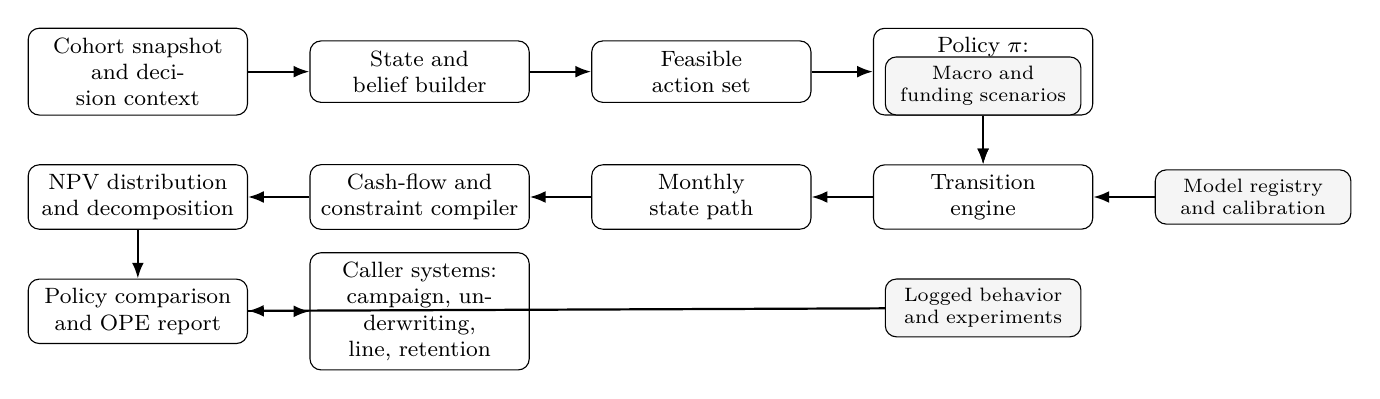
\begin{tikzpicture}[
  node distance=0.62cm and 0.78cm,
  box/.style={draw, rounded corners, align=center, font=\footnotesize,
    minimum height=0.78cm, text width=2.55cm},
  side/.style={draw, rounded corners, align=center, font=\scriptsize,
    minimum height=0.62cm, text width=2.25cm, fill=gray!8},
  arrow/.style={-{Latex[length=2mm]}, thick}
]
\node[box] (cohort) {Cohort snapshot\\and decision context};
\node[box, right=of cohort] (state) {State and\\belief builder};
\node[box, right=of state] (feasible) {Feasible\\action set};
\node[box, right=of feasible] (policy) {Policy $\pi$:\\current, challenger,\\or learned};
\node[box, below=of policy] (trans) {Transition\\engine};
\node[box, left=of trans] (path) {Monthly\\state path};
\node[box, left=of path] (cash) {Cash-flow and\\constraint compiler};
\node[box, left=of cash] (npv) {NPV distribution\\and decomposition};
\node[box, below=of npv] (ope) {Policy comparison\\and OPE report};
\node[box, right=of ope] (caller) {Caller systems:\\campaign, underwriting,\\line, retention};

\node[side, above=of trans] (macro) {Macro and\\funding scenarios};
\node[side, right=of trans] (registry) {Model registry\\and calibration};
\node[side, below=of trans] (logs) {Logged behavior\\and experiments};

\draw[arrow] (cohort) -- (state);
\draw[arrow] (state) -- (feasible);
\draw[arrow] (feasible) -- (policy);
\draw[arrow] (policy) -- (trans);
\draw[arrow] (trans) -- (path);
\draw[arrow] (path) -- (cash);
\draw[arrow] (cash) -- (npv);
\draw[arrow] (npv) -- (ope);
\draw[arrow] (ope) -- (caller);
\draw[arrow] (macro) -- (trans);
\draw[arrow] (registry) -- (trans);
\draw[arrow] (logs) -- (ope);
\end{tikzpicture}
\caption{Policy-simulation interface for the NPV component. The MDP/POMDP layer wraps the existing state, transition, and cash-flow modules so that a declared policy can be simulated, evaluated, and compared before any policy-learning step is considered.}
\label{fig:policy-simulation-interface}
\end{figure}

\hypertarget{required-interfaces}{%
\subsubsection{9.1 Required Interfaces}\label{required-interfaces}}

The component should expose at least four interfaces.

\texttt{simulate\_policy}:

\begin{verbatim}
inputs:
  cohort_snapshot
  policy_id
  baseline_policy_id
  scenario_bundle
  horizon
  valuation_convention
  simulation_controls

outputs:
  expected NPV, incremental NPV, distribution, confidence intervals
  cash-flow decomposition
  constraint-cost decomposition
  path diagnostics
  support/extrapolation warnings
  replay identifiers
\end{verbatim}

\texttt{score\_action\_grid}:

\begin{verbatim}
inputs:
  current state or cohort
  finite action grid
  baseline action
  downstream policy assumption
  scenario bundle

outputs:
  Delta NPV by action
  constraint-cost by action
  sensitivity by macro scenario
  support diagnostics
\end{verbatim}

\texttt{evaluate\_policy\_offline}:

\begin{verbatim}
inputs:
  logged trajectories
  behavior-policy probabilities or estimates
  target policy
  model-based simulator
  estimand definition

outputs:
  direct-method estimate
  importance-sampling estimate where feasible
  doubly robust / weighted doubly robust estimate where feasible
  support and overlap diagnostics
  confidence intervals or conservative bounds
  veto flags
\end{verbatim}

\texttt{register\_policy}:

\begin{verbatim}
inputs:
  policy code or rule specification
  policy version
  action schema
  eligibility/feasibility rules
  intended decision context
  approved use restrictions

outputs:
  policy_id
  reproducibility metadata
  audit and replay metadata
\end{verbatim}

\hypertarget{required-artifacts}{%
\subsubsection{9.2 Required Artifacts}\label{required-artifacts}}

The NPV component should maintain:

\begin{itemize}
\tightlist
\item
  state schema and belief-state schema;
\item
  action schema and feasible-action rules;
\item
  reward and constraint-cost schema;
\item
  transition-model registry;
\item
  policy registry;
\item
  scenario registry;
\item
  simulator calibration report;
\item
  off-policy evaluation report;
\item
  source and claim-support ledger for method claims;
\item
  replay ledger linking a production score to model versions, policy
  versions, scenario versions, and data snapshots.
\end{itemize}

These are not bureaucratic appendices. They are what allow a panel to
verify that a policy comparison means what it says.

\hypertarget{estimation-identification-and-data-requirements}{%
\subsection{10. Estimation, Identification, and Data
Requirements}\label{estimation-identification-and-data-requirements}}

\hypertarget{logged-trajectories}{%
\subsubsection{10.1 Logged Trajectories}\label{logged-trajectories}}

The basic training and evaluation unit should be a customer-month or
account-month trajectory:

\begin{equation}
  \tau_i
  =
  \bigl\{
    (O_{it},b_{it},d_{it},a_{it},p_{it},r_{it},c_{it})
  \bigr\}_{t=0}^{T_i},
  \label{eq:logged-trajectory}
\end{equation}

where $p_{it}$ is the probability that the historical behavior
policy assigned action $a_{it}$ in the observed state. If
$p_{it}$ is unknown, it must be estimated and uncertainty should
be recorded. For deterministic historical policies, the support problem
becomes severe: actions not historically taken in a state cannot be
reliably evaluated from observational data alone.

\hypertarget{identification-assumptions}{%
\subsubsection{10.2 Identification
Assumptions}\label{identification-assumptions}}

The DTR literature makes the key assumptions explicit:

\begin{itemize}
\tightlist
\item
  consistency: the observed outcome under the action actually taken
  equals the potential outcome under that action;
\item
  sequential randomization/no unmeasured confounding: conditional on
  recorded history, the action is as-if randomized with respect to
  future potential outcomes;
\item
  positivity/support: every action considered by the target policy has
  positive probability under the data-generating policy in the relevant
  states;
\item
  no unmodeled interference, or an explicit model of interference.
\end{itemize}

For credit cards, these assumptions are often violated:

\begin{itemize}
\tightlist
\item
  line actions are targeted based on risk, profitability, customer
  complaints, and undocumented policy rules;
\item
  marketing offers are targeted based on propensity models and budget
  constraints;
\item
  approved applicants differ from declined applicants and from
  nonresponders;
\item
  booked accounts differ from approved-but-not-booked accounts;
\item
  account-management actions depend on prior delinquency, utilization,
  manual reviews, operational queues, and regulatory rules;
\item
  competitor actions and macro shocks affect observed behavior but may
  be missing or measured late;
\item
  portfolio capacity and campaign saturation create interference across
  customers.
\end{itemize}

Therefore, a simulator estimate should carry an evidence grade:

\begin{description}[leftmargin=2.1cm,style=nextline]
\item[Grade A] randomized or quasi-randomized support for the decision/action;
\item[Grade B] strong logged-policy support plus credible observed confounding controls;
\item[Grade C] predictive scenario estimate with material identification caveats;
\item[Grade D] extrapolation outside observed support; not usable for decision automation.
\end{description}

\hypertarget{experiments-needed-for-future-rl}{%
\subsubsection{10.3 Experiments Needed for Future
RL}\label{experiments-needed-for-future-rl}}

If the bank wants to use RL rather than only simulate policies, the data
design must change. The relevant experiment is not merely a one-shot A/B
test. Sequential decisions require either:

\begin{itemize}
\tightlist
\item
  randomized holdouts and randomized action grids within policy-safe
  bounds;
\item
  sequential experiments where later randomization depends on prior
  observed history;
\item
  SMART-like designs for selected account-management or retention paths;
\item
  controlled exploration that respects legal, credit, fairness, and
  customer-experience constraints.
\end{itemize}

This does not mean ``randomly increase lines'' or ``randomly harm
customers.'' It means define a policy-safe feasible set first, then
randomize within approved alternatives where the business is genuinely
indifferent or where a controlled experiment is justified.

\hypertarget{off-policy-evaluation-before-policy-improvement}{%
\subsection{11. Off-Policy Evaluation Before Policy
Improvement}\label{off-policy-evaluation-before-policy-improvement}}

Before optimizing policies, the component should evaluate proposed
policies using multiple estimators.

\hypertarget{direct-model-based-evaluation}{%
\subsubsection{11.1 Direct Model-Based
Evaluation}\label{direct-model-based-evaluation}}

The simulator estimates:

\begin{equation}
  \widehat V_{\mathrm{DM}}(\pi)
  =
  \E_{\widehat P}\!\left[
    \sum_{t=0}^{H-1}\beta^t r_t + \beta^H TV_H
    \,\middle|\, \pi
  \right],
  \label{eq:direct-method-value}
\end{equation}

This can have low variance, but it is biased if the transition or reward
model is wrong. It is useful because the NPV component is already a
model-based simulator, but it cannot be the only evidence for
deployment.

\hypertarget{importance-sampling}{%
\subsubsection{11.2 Importance Sampling}\label{importance-sampling}}

If the behavior-policy probability $\mu(a_t\mid h_t)$ and target-policy
probability $\pi(a_t\mid h_t)$ are known or estimable, trajectory
weights can correct for policy mismatch:

\begin{equation}
  w_i(\pi,\mu)
  =
  \prod_{t=0}^{H-1}
  \frac{\pi(a_{it}\mid h_{it})}{\mu(a_{it}\mid h_{it})}.
  \label{eq:trajectory-is-weight}
\end{equation}

Importance sampling is attractive because it directly addresses the
policy mismatch, but it can have very high variance over long horizons.
This is especially relevant for credit-card NPV because the horizon is
long and rare losses matter.

\hypertarget{doubly-robust-and-weighted-doubly-robust-evaluation}{%
\subsubsection{11.3 Doubly Robust and Weighted Doubly Robust
Evaluation}\label{doubly-robust-and-weighted-doubly-robust-evaluation}}

Doubly robust estimators combine a model-based value estimate with
importance-weighted residual corrections. The point is not magic
robustness; the point is bias-variance discipline. Dudik et
al.~establish the idea in contextual bandits, Jiang and Li extend doubly
robust evaluation to finite-horizon RL, and Thomas and Brunskill study
weighted/blended variants for lower mean-squared error.

For the NPV component, the practical requirement is:

\begin{itemize}
\tightlist
\item
  return direct-method, IS/WIS where feasible, and DR/WDR estimates
  where feasible;
\item
  report when weights explode or support is weak;
\item
  report when the model-based estimate and DR estimate materially
  disagree;
\item
  block policy promotion when the evaluation is outside support or
  uncertainty is too wide for the decision.
\end{itemize}

\hypertarget{rl-optimization-roadmap}{%
\subsection{12. RL Optimization Roadmap}\label{rl-optimization-roadmap}}

The MDP/POMDP design makes RL possible, but RL should enter in stages.

\hypertarget{phase-0-mdppomdp-contract}{%
\subsubsection{Phase 0: MDP/POMDP
Contract}\label{phase-0-mdppomdp-contract}}

Deliver:

\begin{itemize}
\tightlist
\item
  state and belief schema;
\item
  action and feasibility schema;
\item
  transition and reward interface;
\item
  constraint-cost schema;
\item
  current-policy simulator;
\item
  policy-comparison reports.
\end{itemize}

No learned policy is required in this phase.

\hypertarget{phase-1-policy-simulation-and-rule-based-challengers}{%
\subsubsection{Phase 1: Policy Simulation and Rule-Based
Challengers}\label{phase-1-policy-simulation-and-rule-based-challengers}}

Evaluate:

\begin{itemize}
\tightlist
\item
  current policy versus declared business alternatives;
\item
  contact versus suppress policies;
\item
  line grids;
\item
  promotion terms;
\item
  retention and inactivity treatments;
\item
  macro-stress policy performance.
\end{itemize}

This phase uses the MDP simulator to make existing policy arguments
coherent.

\hypertarget{phase-2-narrow-offline-policy-improvement}{%
\subsubsection{Phase 2: Narrow Offline Policy
Improvement}\label{phase-2-narrow-offline-policy-improvement}}

Only in decision areas with adequate support:

\begin{itemize}
\tightlist
\item
  contextual bandits for one-shot acquisition/offer selection;
\item
  Q-learning/A-learning style DTR methods for a small number of
  well-defined stages;
\item
  fitted Q iteration for discrete action grids;
\item
  conservative or batch-constrained offline RL for account-management
  actions, with support restrictions.
\end{itemize}

The first serious RL candidate should probably not be a
continuous-action deep RL policy. A discrete action grid for line,
offer, or retention actions is easier to evaluate, easier to constrain,
and easier to explain.

\hypertarget{phase-3-constrained-policy-optimization}{%
\subsubsection{Phase 3: Constrained Policy
Optimization}\label{phase-3-constrained-policy-optimization}}

Move from unconstrained value maximization to constrained MDP
optimization:

\begin{align}
  \max_{\pi}\quad
    & \E[\Delta \NPV^{\pi}] \label{eq:phase3-cmdp}\\
  \text{subject to}\quad
    & \mathcal{C}^{\mathrm{loss}}(\pi)\le \bar C^{\mathrm{loss}}, \notag\\
    & \mathcal{C}^{\mathrm{capital}}(\pi)\le \bar C^{\mathrm{capital}}, \notag\\
    & \mathcal{C}^{\mathrm{funding}}(\pi)\le \bar C^{\mathrm{funding}}, \notag\\
    & \pi(a\mid b,d,M)=0
      \quad \text{for all }a\notin\mathcal{A}(b,d,M), \notag\\
    & \text{fairness, compliance, operational, and customer-experience gates hold.} \notag
\end{align}

This phase should include conservative value estimates, guardrail costs,
support constraints, and independent policy-evaluation reports.

\hypertarget{phase-4-controlled-online-experimentation}{%
\subsubsection{Phase 4: Controlled Online
Experimentation}\label{phase-4-controlled-online-experimentation}}

Deploy only as an experiment:

\begin{itemize}
\tightlist
\item
  small population;
\item
  explicit holdouts;
\item
  pre-specified success and veto criteria;
\item
  common reporting of NPV, losses, complaints, attrition, and fairness
  diagnostics;
\item
  no policy expansion without post-experiment review.
\end{itemize}

\hypertarget{phase-5-recommendation-mode-not-autonomous-mode}{%
\subsubsection{Phase 5: Recommendation Mode, Not Autonomous
Mode}\label{phase-5-recommendation-mode-not-autonomous-mode}}

Even after successful experimentation, the NPV component should
recommend values and policy comparisons. The owning decision system
should decide whether and how to act. This preserves the component
boundary: valuation and policy simulation, not ownership of all bank
decisioning.

\hypertarget{practical-pitfalls-and-required-design-responses}{%
\subsection{13. Practical Pitfalls and Required Design
Responses}\label{practical-pitfalls-and-required-design-responses}}

\hypertarget{post-treatment-leakage}{%
\subsubsection{13.1 Post-Treatment
Leakage}\label{post-treatment-leakage}}

A decision-time state must not include variables caused by the action
being evaluated. For example, post-offer activation, future utilization,
future delinquency, and post-line-change balances cannot be used as if
known at line assignment. The state builder must enforce decision-time
feature cuts.

\hypertarget{selection-bias-through-the-funnel}{%
\subsubsection{13.2 Selection Bias Through the
Funnel}\label{selection-bias-through-the-funnel}}

Prospects, applicants, approved accounts, booked accounts, activated
accounts, and active revolvers are different populations. A single state
transition model fitted only on booked accounts cannot answer
acquisition targeting questions without modeling response, approval,
booking, activation, and censoring.

\hypertarget{unsupported-actions}{%
\subsubsection{13.3 Unsupported Actions}\label{unsupported-actions}}

If historical policy never offered a high line to a certain risk
segment, offline RL cannot reliably prove that high lines are profitable
in that segment. The simulator may generate a scenario, but the evidence
grade must say ``extrapolation.'' BCQ/CQL-style support restrictions are
relevant here.

\hypertarget{reward-misspecification}{%
\subsubsection{13.4 Reward
Misspecification}\label{reward-misspecification}}

Optimizing a scalar reward can create unwanted policies if the reward
omits complaints, servicing burden, fairness risk, liquidity risk, or
future customer harm. The reward should be auditable and constraints
should be explicit.

\hypertarget{simulator-exploitation}{%
\subsubsection{13.5 Simulator
Exploitation}\label{simulator-exploitation}}

An optimizer can exploit errors in the simulator. This is not
theoretical hair-splitting; it is a standard model-based optimization
risk. The design response is to use conservative policy classes, support
constraints, challenger evaluation, stress testing, and randomized
pilots before expansion.

\hypertarget{nonstationarity-and-macro-regimes}{%
\subsubsection{13.6 Nonstationarity and Macro
Regimes}\label{nonstationarity-and-macro-regimes}}

Card behavior changes with unemployment, rates, inflation, liquidity
stress, stimulus, underwriting cycles, and competitive offers. A policy
trained in one regime should be evaluated under multiple scenario
bundles and vintage cohorts.

\hypertarget{interdependence-across-decisions}{%
\subsubsection{13.7 Interdependence Across
Decisions}\label{interdependence-across-decisions}}

Acquisition decisions change the population available for approval;
approval and initial line decisions change later account-management
populations; line policies change spend, utilization, losses, attrition,
and capital. The MDP layer exists precisely to keep these dependencies
visible.

\hypertarget{portfolio-level-constraints-and-interference}{%
\subsubsection{13.8 Portfolio-Level Constraints and
Interference}\label{portfolio-level-constraints-and-interference}}

Marketing budget, line exposure, collections capacity, servicing
capacity, and capital are portfolio-level constraints. If one customer's
action changes capacity for others, independent customer simulation is
incomplete. The first version can approximate portfolio constraints as
scenario inputs and aggregate constraints; later versions may need
portfolio-level state.

\hypertarget{what-should-be-added-to-the-current-proposal}{%
\subsection{14. What Should Be Added to the Current
Proposal}\label{what-should-be-added-to-the-current-proposal}}

The current TeX proposal should eventually receive a new major section,
probably after the path-engine and cash-flow compiler section:

\begin{quote}
\textbf{MDP/POMDP Policy-Simulation Layer}
\end{quote}

That section should include:

\begin{enumerate}
\def\labelenumi{\arabic{enumi}.}
\tightlist
\item
  The formal state/action/transition/reward/constraint notation from
  this note.
\item
  A diagram showing how the existing NPV modules become the transition
  and reward machinery of the MDP.
\item
  A statement that the first production use is policy simulation and
  policy evaluation, not autonomous RL.
\item
  A subsection on POMDP belief states for wallet share, adoption,
  liquidity stress, and latent behavior.
\item
  A subsection on action feasibility and support restrictions.
\item
  A subsection on off-policy evaluation and evidence grades.
\item
  A phased RL roadmap.
\item
  A reviewer-facing table with source support, but only after prose
  explanation and in a readable form.
\end{enumerate}

The literature review should also be amended so that RL/MDP material is
not bolted onto the end. The better organization is:

\begin{enumerate}[leftmargin=*]
\item Customer NPV is a sequential valuation problem.
\item Sequential valuation needs states, actions, transitions, rewards, constraints, and policies.
\item The existing spend/loss/balance/attrition literature supplies transition modules.
\item The MDP/POMDP literature supplies the integration grammar.
\item The DTR/OPE/offline-RL literature supplies the identification and evaluation discipline.
\end{enumerate}

That is integration, not a separate RL appendix.

\hypertarget{source-support-ledger}{%
\subsection{15. Source-Support Ledger}\label{source-support-ledger}}

This ledger records what the inspected sources support. It should be
carried into the proposal's citation discipline if this note is
integrated.

Sutton and Barto, \emph{Reinforcement Learning: An Introduction}, 2018.
Local artifact:
\artifactpath{docs/credit-card-npv-mdp-rl-sources/sutton_barto_rl_2018.pdf}.
Classification: foundational. The inspected sections support the basic
RL vocabulary used in this note: policy, reward, value function, model,
state, and MDP framing. They support saying that a customer-value
problem with delayed effects can be represented as a sequential decision
problem. They do not support saying that RL is safe or effective for
production credit-card decisioning.

Kaelbling, Littman, and Cassandra, 1998. Local artifact:
\artifactpath{docs/credit-card-npv-mdp-rl-sources/kaelbling_littman_cassandra_pomdp_1998.pdf}.
Classification: foundational and direct method. The inspected sections
define the POMDP tuple, explain that belief states are probability
distributions over latent states, and state the sufficiency logic under
a correct model. This supports using belief states for latent wallet
share, liquidity stress, risk, and preferences. It does not support
claiming that exact POMDP solution is feasible for a high-dimensional
bank portfolio.

Schulte et al., 2012. Local artifact:
\artifactpath{docs/credit-card-npv-mdp-rl-sources/schulte_q_a_learning_dynamic_treatment_2012.pdf}.
Classification: direct method. The inspected sections define dynamic
treatment regimes, histories, SMART data, consistency, sequential
randomization, positivity, Q-learning, and A-learning. This supports the
identification discussion and the need for randomized or well-supported
sequential action histories. It does not establish card-specific
treatment effects.

Laber et al., 2010. Local artifact:
\artifactpath{docs/credit-card-npv-mdp-rl-sources/laber_qian_lizotte_pelham_murphy_dtr_inference_2010.pdf}.
Classification: direct method. The inspected sections discuss DTR
construction, Q-learning, and inference/nonregularity challenges. This
supports warning that optimal sequential-regime inference is delicate
and that naive confidence statements around Q-learning can be
misleading. It does not support bank-card effectiveness claims.

Ernst et al., 2005. Local artifact:
\artifactpath{docs/credit-card-npv-mdp-rl-sources/ernst_fitted_q_iteration_2005.pdf}.
Classification: direct method. The inspected sections describe
batch-mode four-tuples and fitted Q iteration through supervised
regression and Bellman backups. This supports fitted Q iteration as a
candidate method for discrete action grids and logged trajectories. It
does not establish production readiness in financial services.

Dudik et al., 2011. Local artifact:
\artifactpath{docs/credit-card-npv-mdp-rl-sources/dudik_doubly_robust_policy_evaluation_2011.pdf}.
Classification: direct method. The inspected sections discuss
contextual-bandit policy evaluation, direct-method bias,
inverse-propensity variance, and doubly robust estimation. This supports
DR logic for one-shot card decisions and offer selection. It does not by
itself support full sequential-card NPV evaluation.

Jiang and Li, 2015/2016. Local artifact:
\artifactpath{docs/credit-card-npv-mdp-rl-sources/jiang_li_doubly_robust_ope_rl_2015.pdf}.
Classification: direct method. The inspected sections discuss
finite-horizon off-policy value evaluation, model-based and
importance-sampling approaches, and a doubly robust estimator. This
supports using DR OPE as part of sequential policy evaluation. It does
not support automatic policy approval without support checks.

Thomas and Brunskill, 2016. Local artifact:
\artifactpath{docs/credit-card-npv-mdp-rl-sources/thomas_brunskill_data_efficient_ope_2016.pdf}.
Classification: direct method. The inspected sections discuss WDR/MAGIC,
mean-squared-error trade-offs, and confidence interval issues. This
supports using multiple OPE estimators and uncertainty reporting before
deployment. It does not imply that OPE proves causal validity when
logging policy or support assumptions fail.

Levine et al., 2020. Local artifact:
\artifactpath{docs/credit-card-npv-mdp-rl-sources/levine_offline_rl_tutorial_2020.pdf}.
Classification: survey/tutorial. The inspected sections define offline
RL as learning from a static dataset, emphasize counterfactual queries,
and identify distribution shift as a core difficulty. This supports
treating logged bank data as an offline-RL setting with serious
extrapolation risk. It is tutorial support, not a theorem for this
specific bank problem.

Fujimoto et al., 2018/2019. Local artifact:
\artifactpath{docs/credit-card-npv-mdp-rl-sources/fujimoto_bcq_2018.pdf}.
Classification: direct method. The inspected sections explain
fixed-batch RL failure from extrapolation error and motivate
batch-constrained policies. This supports action-support restrictions
and caution around unseen actions. It does not imply that BCQ is the
preferred production method.

Kumar et al., 2020. Local artifact:
\artifactpath{docs/credit-card-npv-mdp-rl-sources/kumar_conservative_q_learning_2020.pdf}.
Classification: direct method. The inspected sections discuss offline
distribution shift, out-of-distribution actions, overestimated Q-values,
and conservative lower-bound value estimates. This supports conservative
offline RL as a candidate method when support is limited. It does not
imply that CQL solves all bank policy risk.

Achiam et al., 2017. Local artifact:
\artifactpath{docs/credit-card-npv-mdp-rl-sources/achiam_constrained_policy_optimization_2017.pdf}.
Classification: direct method. The inspected sections define constrained
MDPs with auxiliary costs and limits. This supports modeling loss,
capital, funding, fairness, compliance, and operational quantities as
constraints rather than folding everything into reward. It does not
imply that CPO itself should be used in production.

Alfonso and Sanchez, 2023/2024. Local artifact:
\artifactpath{docs/credit-card-npv-mdp-rl-sources/alfonso_sanchez_credit_limit_rl_2023.pdf}.
Classification: direct domain example. The inspected sections formulate
credit-limit management as an MDP, define line actions, and define
reward as expected profit net of provisions over a short horizon. This
supports saying that card line management can naturally be formulated as
an MDP. It does not justify generalizing the method to all US
retail-bank card decisions.

Trench et al., 2003, ``Managing Credit Lines and Prices for Bank One
Credit Cards.'' Local artifact:
\artifactpath{docs/credit-card-npv-mdp-rl-sources/trench_pederson_lau_ma_wang_nair_bank_one_portico_2003_SOURCE_BLOCKED.html}.
Classification: high-priority source-blocked direct domain precedent.
Crossref metadata for DOI \texttt{10.1287/inte.33.5.4.19245} identifies
an INFORMS Interfaces article on a Bank One PORTICO system using MDPs to
choose card APRs and credit lines with an NPV objective. The publisher
PDF was blocked by Cloudflare in this environment, so the article should
not be used as inspected technical support until retrieved through a
library or licensed source.

Tkachenko, 2015. Local artifact:
\artifactpath{docs/credit-card-npv-mdp-rl-sources/tkachenko_crm_clv_deep_rl_2015.pdf}.
Classification: empirical example. The inspected sections frame CRM/CLV
as an MDP with customer state, marketing action, reward, and value
interpreted as customer lifetime value. This supports the customer-value
analogy. It does not provide production proof or banking-specific
validation.

Murphy, 2003. Local artifact:
\artifactpath{docs/credit-card-npv-mdp-rl-sources/murphy_optimal_dynamic_treatment_regimes_2003_SOURCE_BLOCKED.html}.
Classification: source-blocked. The local file is an HTML failure page,
not an inspected PDF. It may be used only as bibliographic context if
separately cited from the existing bibliography. It should not be used
as checked technical support until the real source is obtained.

\hypertarget{remaining-literature-and-evidence-gaps}{%
\subsection{16. Remaining Literature and Evidence
Gaps}\label{remaining-literature-and-evidence-gaps}}

This note is source-grounded but not complete as a final literature
review. Before panel submission, the integrated proposal should add or
verify:

\begin{itemize}
\tightlist
\item
  Puterman's MDP text or another checked MDP reference for
  operations-research readers;
\item
  Altman's constrained-MDP book or a checked accessible source if CMDP
  theory is emphasized;
\item
  Rust-style structural dynamic discrete-choice literature if the
  proposal argues for structural estimation of customer behavior;
\item
  additional direct financial-services sequential-decision papers if
  available through licensed databases;
\item
  retraction/erratum and publication-version checks for all downloaded
  PDFs;
\item
  citation and venue metadata with access dates, if the panel expects
  bibliometric coverage;
\item
  internal bank data evidence: replay calibration, policy support
  diagnostics, and examples of how current policies generate observed
  action variation.
\end{itemize}

These gaps do not invalidate the design conclusion. They are the next
source-hardening tasks before the MDP/RL section is folded into the main
proposal.

\hypertarget{bottom-line}{%
\subsection{17. Bottom Line}\label{bottom-line}}

The right design is a POMDP-aware MDP simulator embedded inside the NPV
component. It should make the following contract explicit:

\begin{equation}
  (b_t,\mathcal{A}_t,\pi,s)
  \longrightarrow
  \{X_{t+h}\}_{h=1}^{H}
  \longrightarrow
  \{r_{t+h},c_{t+h}\}_{h=0}^{H-1}
  \longrightarrow
  \bigl(\Delta\NPV^{\pi},\text{ policy-evaluation evidence}\bigr).
  \label{eq:bottom-line-contract}
\end{equation}

This design allows the bank to simulate a policy forward, compare
policies coherently, and eventually apply RL or dynamic-treatment-regime
methods where the data support them. It also prevents the dangerous
shortcut: optimizing a collection of disconnected predictive models as
if they formed a valid sequential decision system.

\end{document}
